\section{The Analysis Framework}
\label{sec:factory}

\noindent
To systematically analyze different scheduling policies in an apples-to-apples manner,
we implement a flexible LLM scheduling analysis framework---{\sys}. 
The key drivers for {\sys} are twofold:
(1) Existing policies are buried in concrete (both open-source and closed-source) implementations of different serving systems, 
making it
hard to compare them in an apples-to-apples manner.
For example, the Go implementation of vLLM's policy
on AIBrix~\cite{aibrix} is 6.2\,$\times$ faster than vLLM's Python implementation~\cite{vllm-code}
due to a later confirmed performance bug~\cite{vllm-bug}.
Meanwhile,
our Rust-based implementation achieves a further 1.2\,$\times$ speedup over AIBrix with the same 
vLLM policy.
(2) A unified framework simplifies implementing new policies for comparison:
Though complex, all existing policies boil down to computing scheduling scores
based on the indicators of the instances.
By providing a unified indicator factory, 
our framework allows exploring policies with a few lines of code (described below). 
%With \TODO{3596} lines of code, we reimplemented the \TODO{TTFT prediction logic}\ described in Mooncake's paper~\cite{305212}.

%Note that we have carefully calibrated {\sys}'s performance with open-source global router implementations. 

\begin{figure}[!t]
%        \hspace{-2mm}
        \begin{minipage}{1\linewidth}
        \centering
        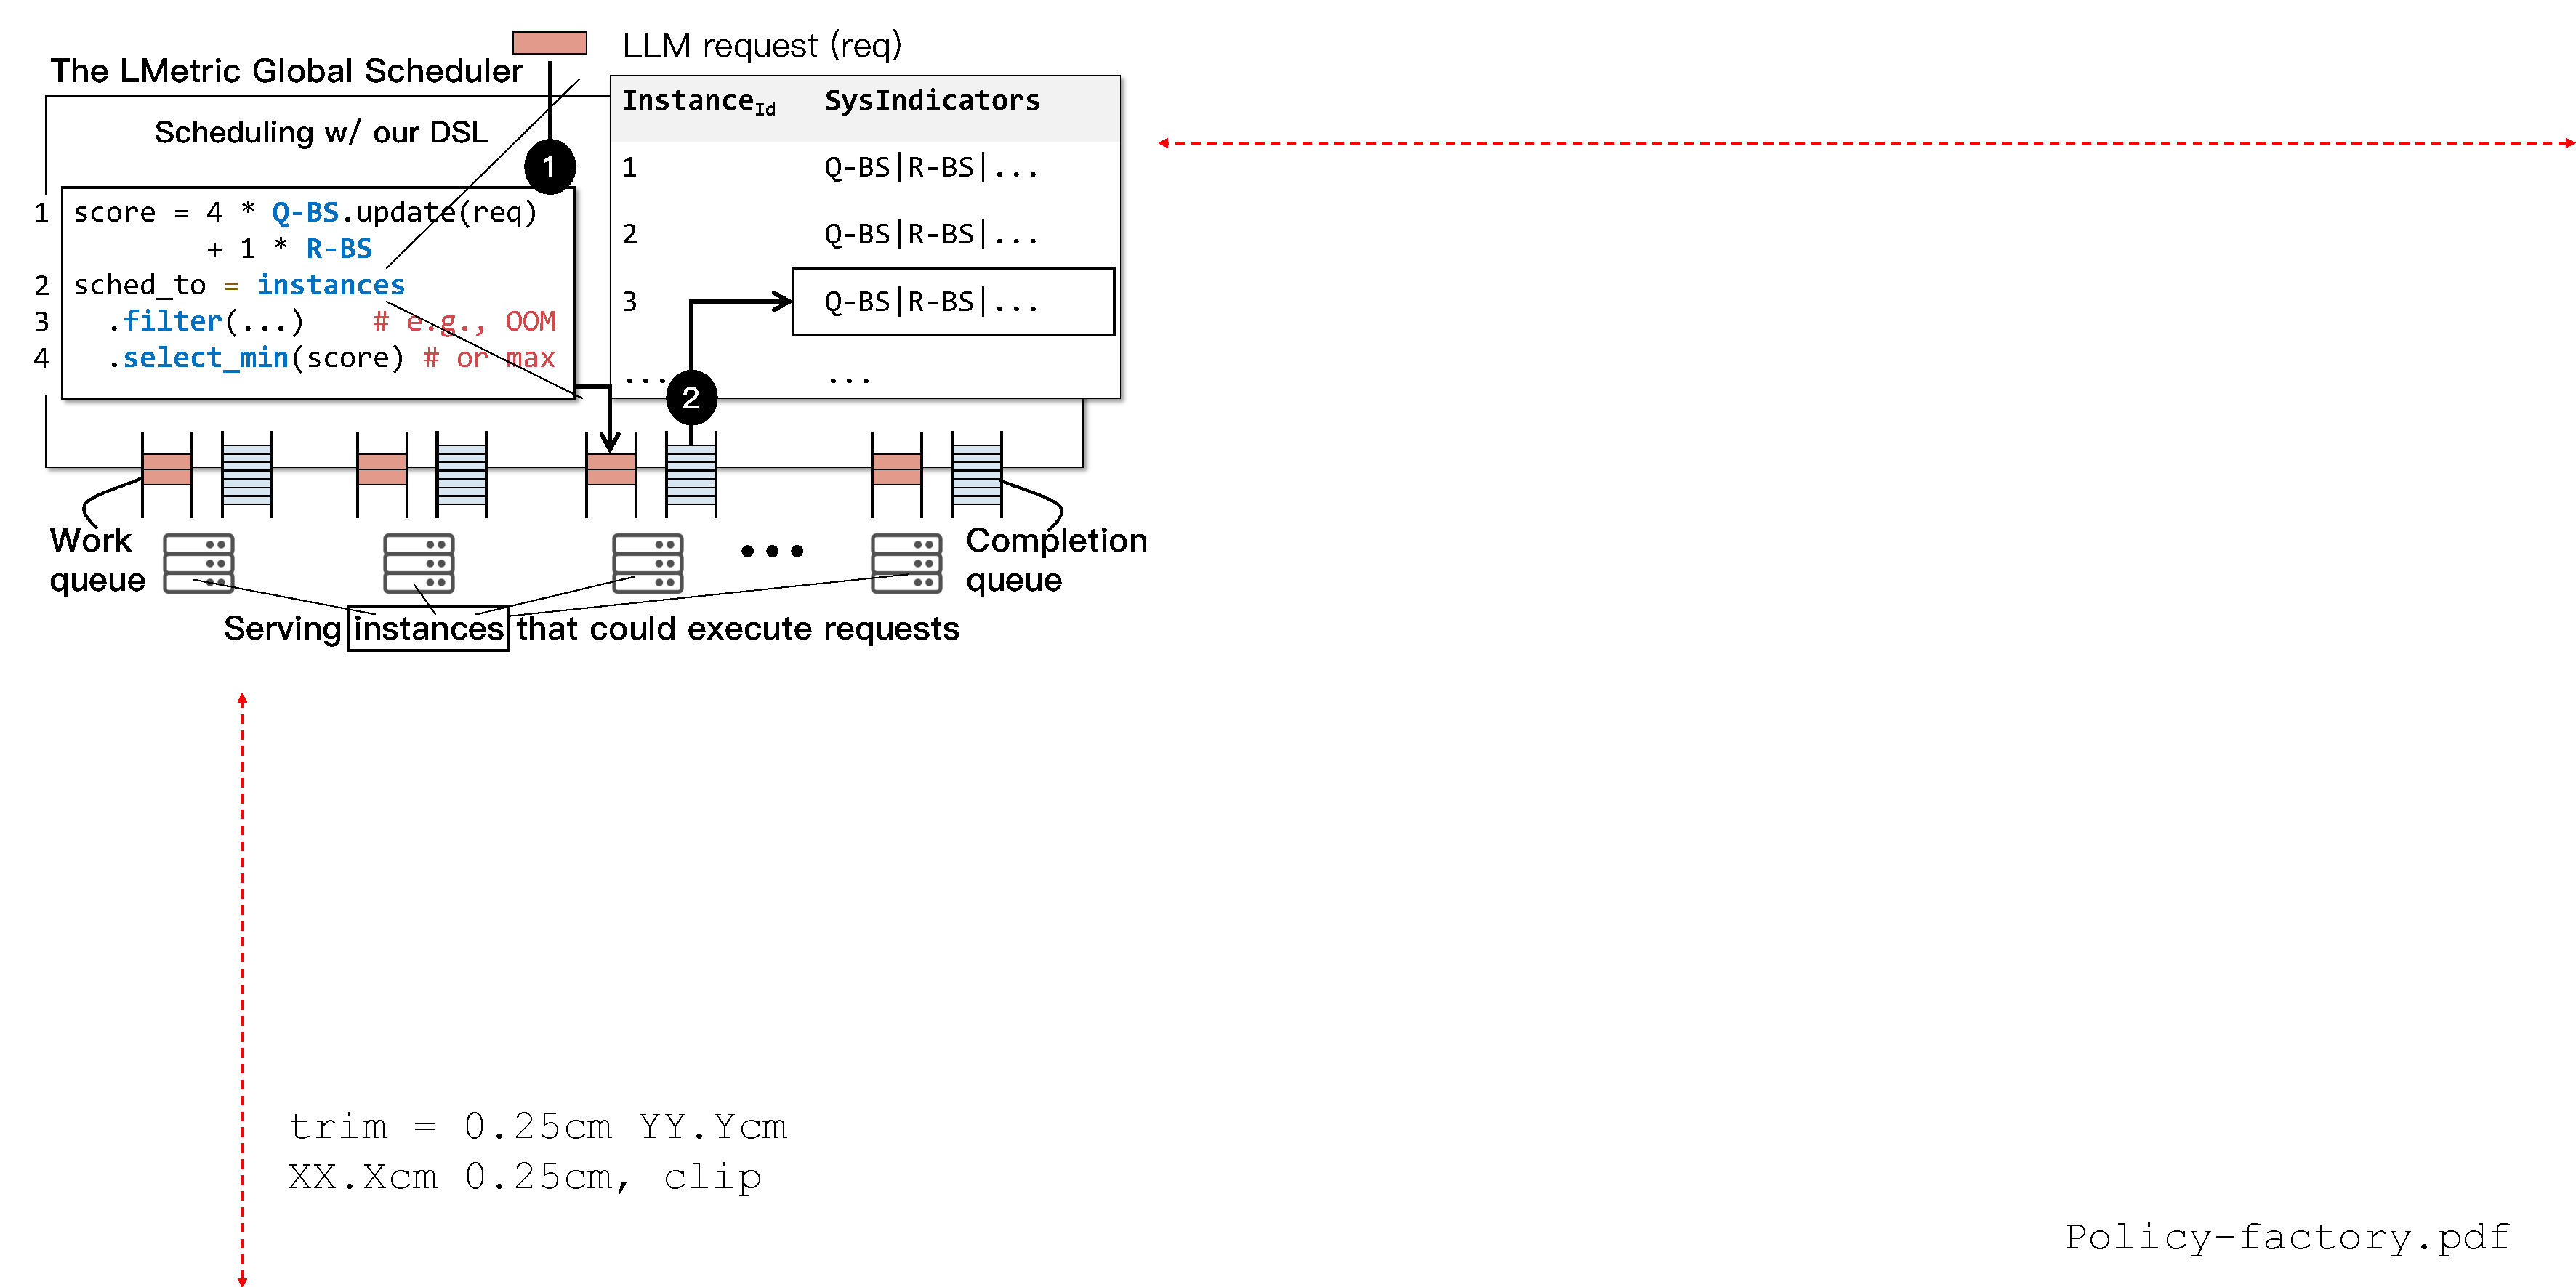
\includegraphics[width=0.95\linewidth, trim=0.25cm 14.75cm 33cm 0.25cm, clip]{figs/policy-factory.pdf}
        \end{minipage} \\[5pt]
        \begin{minipage}{1\linewidth}
        \caption{\small{%
        The system architecture of the {\sys} metric factory
        and its programming model for scheduling algorithms.
        }}
        \label{fig:factory}
        \end{minipage} \\[-10pt]
        \end{figure}

\stitle{Indicator factory. \,}
{\sys} is a standalone inference router implemented in Rust that can collaborate with any LLM serving engine.
Its key component---as shown in {\fig{fig:factory}}---is an \emph{indicator factory}
that automatically collects and computes the indicators (if necessary) required for different scheduling policies.
Choosing Rust enables {\sys} to be extremely efficient and robust.
For high scalability, indicator collection is piggybacked on
the receipt of responses from the instances.
For example, {\sys} maintains a long-lived connection to each vLLM instance, and
when vLLM sends a response back, {\sys} extracts the required indicators from the response header
and updates the corresponding indicators in the factory.

\stitle{Programming model.  \,}
{\sys} provides a simple API to implement different scheduling policies.
Specifically, all policies essentially first compute a score for each instance
and then route the request to the instance with the best (e.g., minimum or maximum) score.
Our API allows developers to define score functions over per-instance symbolic indicators supported by our factory 
with a few lines of expressions.
Line 1 in {\fig{fig:factory}} shows a concrete policy adopted by vLLM~\cite{vllm-code}:
it computes the score as a weighted sum of \texttt{Q-BS} (queued batch size---the number of queued requests in an instance's queue)
and \texttt{R-BS} (the number of running requests on the instance).
With the defined score function,
when deciding where to route a new request (line 4),
{\sys} first retrieves and computes the concrete indicator values from the indicator factory in parallel,
then derives the scores for all instances, and finally routes the request to the instance with the minimum score.
%To the best of our knowledge, all known LLM scheduling policies
%can be expressed in this pattern (see Appendix~\ref{} \TODO{xx}).

